\chapter{Einleitung[EK]}
In der heutigen digitalisierten Welt fallen Tag für Tag immer mehr Daten an, die schiere Masse wird für immer mehr Stakeholder jener zu einem Problem. Denn allein die Menge ist zu groß, um unaufbereitet aus dieser, in einem vernünftigen und logisch aufgebauten Prozess, Schlüsse ziehen zu können.
\par
Mit der Jahrtausendwende kam es zu einem „Goldrausch“ der Daten, welcher mit dem Aufstieg des Internets und dem schnellen Wandel von einer zahlungspflichtigen Softwarewelt zu einer für die Nutzer „frei“ zu Verfügung stehenden Software losgetreten wurde. Dadurch veränderte sich ein beachtlicher Teil der Finanzierungsüberlegungen der davon betroffenen Unternehmen: Nicht mehr direkt selbst sollte der Nutzer diese Dienste monetär bezahlen, sondern durch seine Daten.
\par
So gehandhabt in der Welt, welche für die breite Öffentlichkeit zugänglich und ersichtlich ist. Jedoch trug vor allem dieser Wandel einen beachtlichen Teil dazu bei, dass Daten nun zur “Währung” des neuen Jahrhunderts wurden. Nicht nur im B2C tat sich viel, sondern auch im B2B. So wurden im Laufe der fortschreitenden Digitalisierung immer mehr Daten digital gesammelt. Nun waren einst schwer und aufwendig zu analysierende Daten digital zugänglich. Somit wurde die Brücke erschaffen, welche es Softwarelösungen ermöglichen sollte diese Daten nun zu extrahieren und Entscheidungsprozesse aus dem daraus gewonnen Wissen damit zu Unterstützen.
\begin{figure}[H]
    \centering
    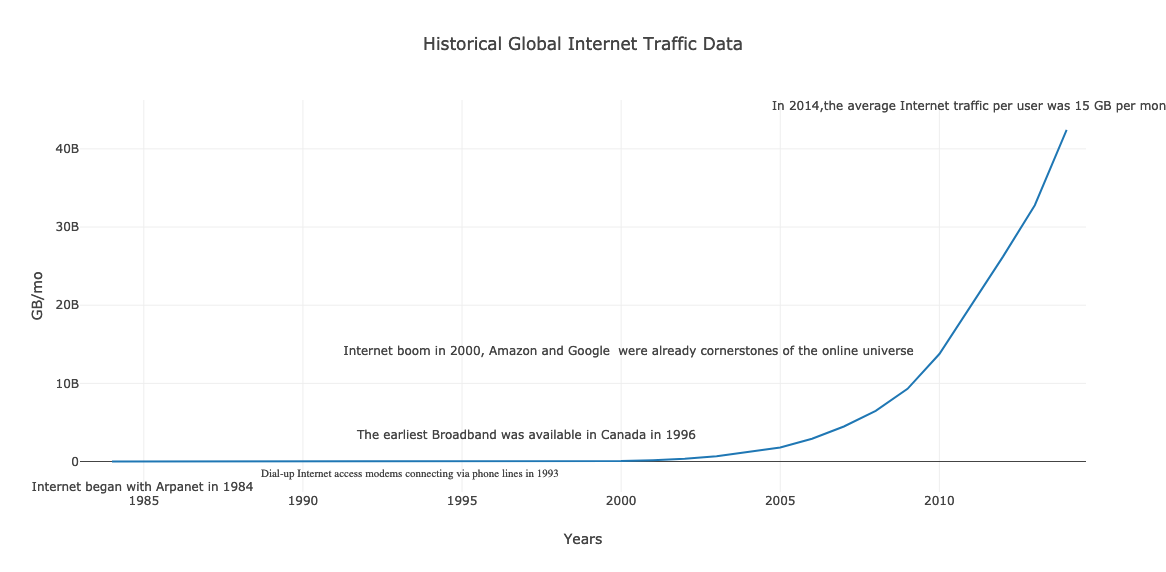
\includegraphics[scale=0.35]{images/Gfk-01.png}
    \caption{Internetverkehr in den letzten Jahrzehnten (02.04.2020)}
    \url{https://plot.ly/~QY/3.embed}
\end{figure}
Der Graph veranschaulicht, wie stark das Datenaufkommen in den letzten Jahrzehnten eine rasante Steilkurve angelegt hat und somit Rückschlüsse darauf ziehen lässt, mit welchen immensen Datenmengen wir es heutzutage zu tun haben. Und das erst bei einer relativ kurzen historischen Periode.
\par
Heute im 2. Jahrzehnt dieses Jahrhunderts ist eine stetig wachsende Wichtigkeit dieses neu begründeten Bereichs der Daten-Analyse eminent. Dadurch ist auch für unseren Auftraggeber, die Firma MIC, ein aufkommendes Interesse in diesen Bereich entstanden. Aus diesem Anlass wurde uns die Aufgabe zu teil, uns mit der Thematik auseinanderzusetzen und Unternehmungen in diesen Bereich mit anzustoßen.
\newpage
\section{Ausgangslage}
Das Thema des ETL-Prozesses und Datenanalyse ist daher für uns von Interesse, da es sich um eine Thematik handelt, welche in unserer HTL-Ausbildung wenig vorkommt. Die Erarbeitung von etwas für uns komplett Neuem steht dabei klar im Fokus. 

Bei ETL handelt es sich keinesfalls um ein neues Konzept. Viele bereits vorhandene ETL-Tools erfordern jedoch eine klare Einlassung auf ein bestimmtes Unternehmen, was für eine Abhängigkeit sorgt. Werden also schnell bestimmte Funktionalitäten gebraucht, welche nicht vom Anbieter angeboten werden, oder welche nicht zu kosteneffizienten Wegen zu erreichen sind, hat man ein Problem. Mithilfe dieser Arbeit sollte eine unabhängige Basis gelegt werden. 

\subsection{Verwandte Arbeiten und Projekte}
Unsere Arbeit ist nicht die Einzige, welche sich mit der Thematik des ETL-Prozesses und deren Analyse auseinandersetzt. Neben unserer Arbeit hat die MIC auch intern an einem Prototypen im Bereich der ETL-Prozesse und Datenanalyse gearbeitet. Im Unterschied zu unserem Projekt sollte dieser aber restriktivere Anforderungen in der Technologiewahl einhalten. 
\vspace{5mm}\par
Darüber hinaus wurde uns als Einführung in die Materie die Masterarbeit „Entwicklung flexibler und erweiterbarer ETL- Systeme für die internationale Zollabwicklung“ aus dem Jahre 2018 von Dominik Schachner, BSc, zur Verfügung gestellt. Auch diese Arbeit wurde im Rahmen einer Kooperation mit der MIC erstellt.
\vspace{5mm}\par
ETL-Lösungen müssen aber nicht umbedingt selbst implementiert werden. Je nach Bedarf und Datenquelle bieten verschiedenste Anbieter, wie IBM, Amazon, Google, eigene Lösungen an.
\par
Der Unterschied und Ansatz unserer Arbeit liegt darin möglichst modular aufgebaut zu sein und so eine einfache Erweiterbarkeit bieten zu können.


\newpage
\section{Struktur der Diplomarbeit}
In der Aufgabenstellung gehen wir darauf ein, was die Erwartungen der beiden kooperierenden Parteien - der Firma MIC und uns - für die Arbeit war.
\vspace{5mm}\par
Darauf folgend legen wir die theoretischen Grundlagen, auf welchen unsere Arbeit beruht, dar.
Dies geschieht in der logischen Reihenfolge des Datenflusses, beginnend von den Datenquellen über die Verarbeitung bis zur Darstellung.
\vspace{5mm}\par
Im Kapitel Werkzeuge legen wir da, welche Mittel wir für diese Arbeit verwendet haben. Im Unterkapitel Arbeitswerkzeuge werden die Werkzeuge beschrieben, welche uns bei der Entwicklung geholfen haben, aber selbst kein Bestandteil des Prototyps an sich sind. Bei Technologien werden jene erläutert, welche Teil des Prototyps sind. So ist Docker Teil der Technologien, da die einzelnen Bestandteile des Prototyps systemunabhängig über geschriebene Dockerfiles erst zum Zusammenschluss kommen. AWS hingegen ist nur die Plattform, welche die Möglichkeit veranschaulichen soll, dass der Prototyp auf einem Cloud-Service lauffähig gemacht werden kann, indem dieser durch Docker eine Systemunabhänigkeit erreicht.
\vspace{5mm}\par
In der “Praktischen Umsetzung” legen wir unseren Schaffensprozess für den Prototypen dar. 
Dieses Kapitel behandelt dafür vier Punkte. Erstens beschreibt es die Konfiguration und Einrichtung der Werkzeuge. Zweitens erläutert es aufkommenden Hürden bei der Realisierung. Drittens beschreibt es den Code in den geschriebenen Modulen. Viertens legt es argumentativ die Entscheidungsprozesse dar.
\vspace{5mm}\par
Zu guter Letzt legen wir im Fazit unsere Meinung und Erfahrungswerte zu dieser Arbeit dar.

\section{Projekt und Dokumentation}
Der Prototyp, seine einzelnen Module, die CI-Tätigkeiten und die Dokumentation sind online in folgendem Repository zu finden:
\href{https://github.com/soyabeantec/AKK}{https://github.com/soyabeantec/AKK}